\documentclass[]{article}
\usepackage{graphicx}
\usepackage{amsmath}

%opening
\title{Distinguishing Noise from Normative Determinants: A Comparison of Four Methods}
\author{Mao Hu \\ Duke University \\ mao.hu@duke.edu \and Jonathan H. Morgan \\ Department of Sociology \\ Duke University \\ jhm18@duke.edu}


\begin{document}

\maketitle

\section{Abstract}

Cross-cultural differences in the processing of interactions have interested social psychologists for decades (Heise 2010a). Smith, Matsuno, and Ike (2001) use affect control theory to identify cross-cultural differences. Although these studies indicate that cultures influence how people appraise situations, Heise's forthcoming study comparing procedures for determining normative sentiments has prompted researchers to re-examine the extent of these cultural differences in interaction.

This work contributes to the debate by examining two Bayesian methods for identifying predictors of normative sentiment changes and comparing them to stepwise regression and the ANOVA procedures documented by Heise.  We evaluate these procedures with reference to a simulated baseline informed by a panel study of affective meanings, allowing us to rule out confounding effects resulting from individual differences or the data collection process.  

\section{Example Analysis}

To provide context, we discuss an analysis comparing stepwise, ANOVA, and two Bayesian Model Averaging procedures, implemented in the \verb+BMA+ (Bayesian Model Averaging) and \verb+BMS+ (Bayesian Model Sampling) packages in \verb+R+ (Feldkircher 2009).  Our analysis evaluates the ability of the procedures to identify variable combinations that predict impression change (the difference between out-of-context and in-context meanings resulting from an event).

 Meanings are operationalized as three dimensional vectors representing the evaluation, potency, and activity of a given concept. \footnote{For more information on the modeling of meanings and events, please refer to Heise’s (2010b) book, \underline{Expressive Order: Confirming Sentiments in Social Action.}} Events are operationalized as actor, behavior, object combinations (ABOs), or who (the actor) did what (the behavior) to whom (the object).  We model impression change using a linear equation consisting of the main effects of each component (A, B, and O) for each dimension (9 parameters), second order interactions, and cross-word third order interactions (sixty-three parameters in all).
 

We take Smith-Lovin's (1988) estimates for impression-change equations as the ``ground truth" reference model.  From this model, we generated 100 simulations consisting of 400 events whose covariance structure is similar to the Duke 2010 data set.  For each simulation, we trained all four methods on half of the corpus.  \textbf{Table 1} and \textbf{Figure 1} summarize the results.

\begin{table}[h]
\caption{Comparison of the Average Performance of the Procedures}
\begin{tabular}{l r r r r}
Procedures & True-Positive & False-Positive & Sensitivity & Iden. Error \\ \hline
Stepwise & 10 & 15 & 10/15 & 15/25 \\
ANOVA & 4 & 1 & 4/15 &  1/5 \\
Bayesian Model Averaging & 6 & 2 & 6/15 & 2/8 \\
Bayesian Model Sampling & 5 & 1 & 5/15 & 1/6 \\ \hline
\end{tabular}
Values rounded up to the nearest whole number\\
Sensitivity $= \frac{\text{\# True Positive}}{\text{\#  True Predictors}} $\\
Iden. Error $= \frac{\text{\# False Positive}}{\text{\#  Identified as positive}} $ 
\end{table}

The reference model has fifteen true predictors. Interpreting the table, the second column lists predictors that were both true (in the reference model) and identified by the procedure; the third column lists predictors that were not true but were identified by the procedure; the fourth column lists the proportion of ABO interactions correctly identified by the procedure over the number that were actually true; the fifth column lists the proportion of ABO interactions incorrectly identified over those correctly identified. 


Our analysis confirms Heise's (forthcoming findings) that the ANOVA procedure is more specific.  Stepwise regression identified 1.5 times more false positives than true positives. Bayesian Model Sampling identified 1 false positive for every five true positives. Thus, we show that the Bayesian procedures have higher specificity than stepwise regression and higher sensitivity than ANOVA.

\begin{figure}[h]
\caption{Comparison of the Distribution of the Procedure Performance}
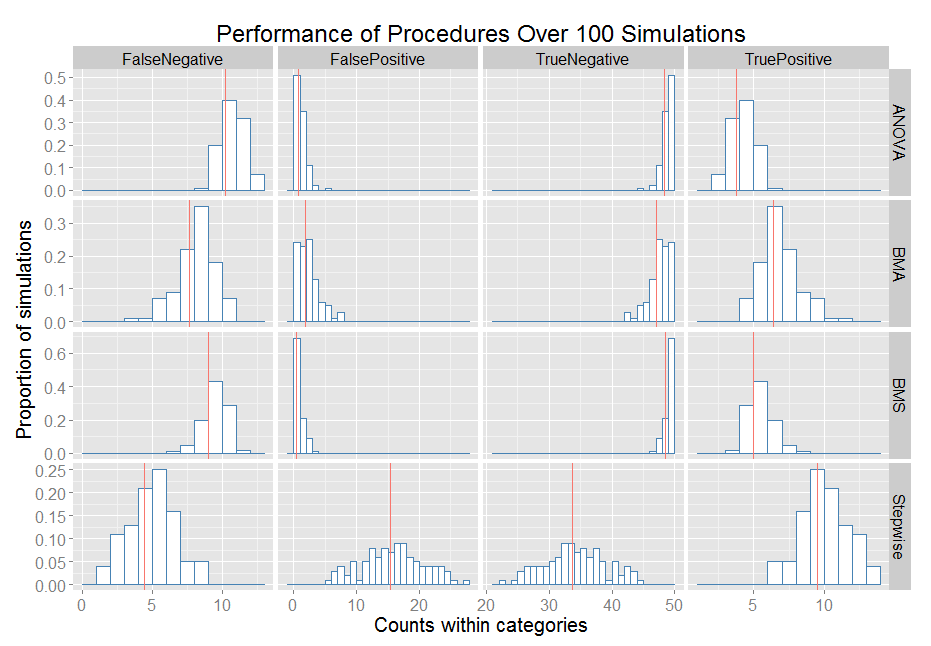
\includegraphics[width=1.1\textwidth]{fig1.png}
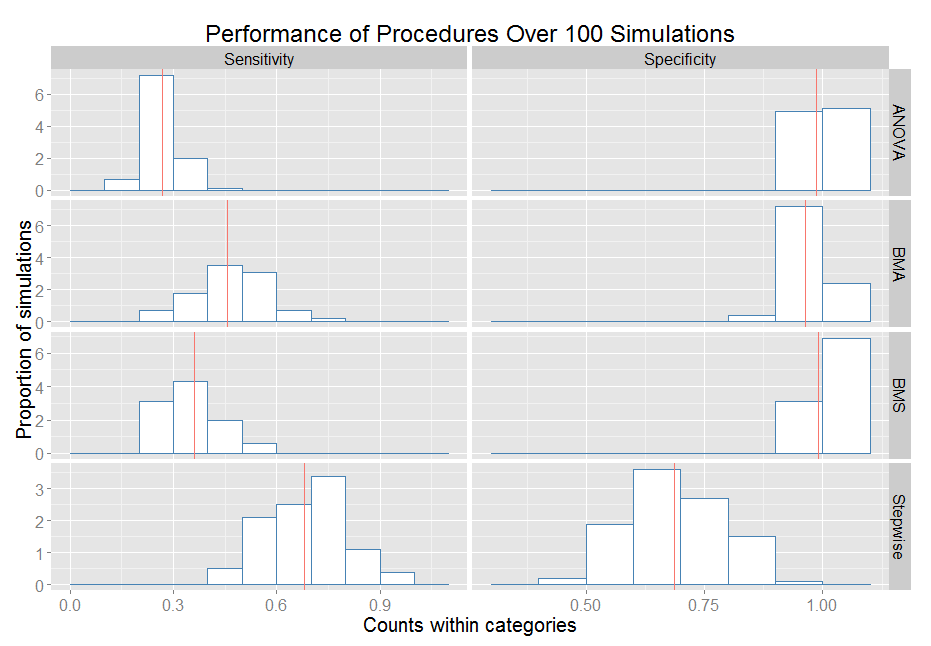
\includegraphics[width=1.1\textwidth]{fig2.png}
\end{figure}

\begin{figure}[h]
\caption{Correlation Structure of Simulated Data (Left) vs. Duke '10 Data (Right)}
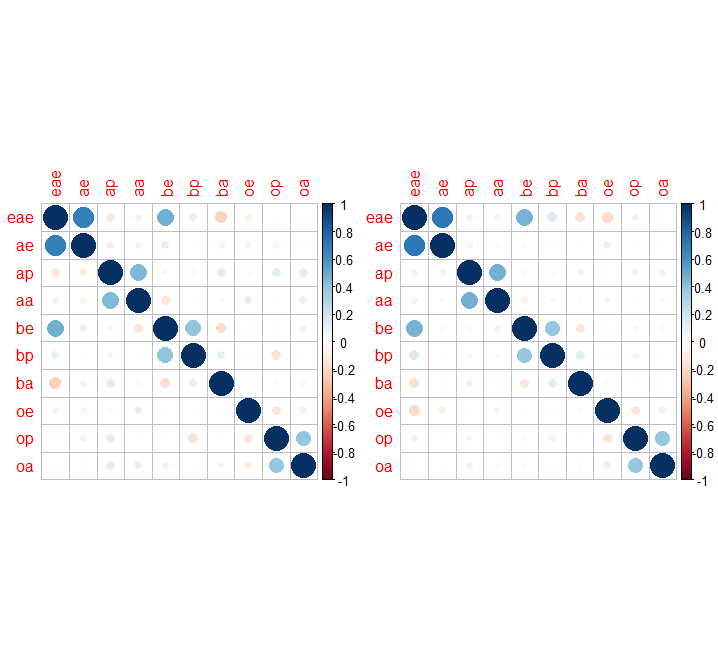
\includegraphics[width = 1.1\textwidth]{structure.png}
\end{figure}




\begin{thebibliography}{9}

\bibitem{bms}
Feldkircher, M. and S. Zeugner (2009): Benchmark Priors Revisited: On Adaptive Shrinkage and the Supermodel Effect in Bayesian Model Averaging; IMF Working Paper 09-202

\bibitem{heise1}
	Heise, David R.
  2010a. Expressive Order: Confirming Sentiments in Social Action. Bloomington, IN, Springer.
  
\bibitem{heise2}
  Heise, David R. 2010b. Surveying Cultures: Discovering Shared Conceptions and Sentiments. Hoboken, NJ, Wiley.
  
\bibitem{heise3}
  Heise, David R. forthcoming. "Determinants of Normative Processes: Comparison of Two Empirical Methods of Specification." Quality and Quantity.
  
\bibitem{smith1}
  Smith, Herman W, Takanori Matsuno, and Shuuichirou Ike. 1994. "The Affective Basis of Attributional Processes among Japanese and Americans." Social Psychology Quarterly 64(2): 180-194.
  
    \bibitem{smith2}
  Smith-Lovin, Lynn. 1988. “Impressions from Events”, pp. 35-71 in Lynn Smith-Lovin and David R. Heise, ed. Analyzing Social Interactions: Advances in Affect Control Theory. New York, NY: Gordon and Breach Science Publishers.
  
  
\end{thebibliography}

\end{document}
